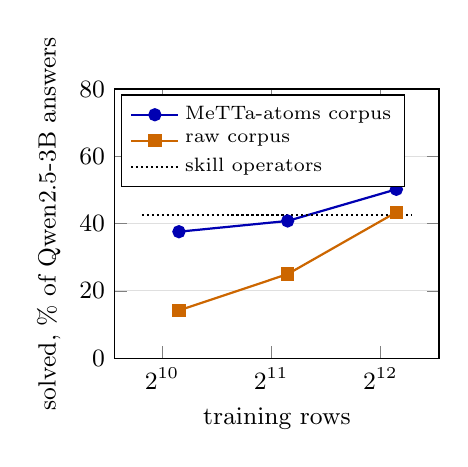
\begin{tikzpicture}
\begin{axis}[width=0.47\linewidth, height=5.0cm, xmode=log, log basis x=2, xlabel={training rows}, ylabel={solved, \% of Qwen2.5-3B answers},
  ymin=0, ymax=80, ymajorgrids, grid style={gray!25}, legend style={font=\scriptsize, at={(0.02,0.98)}, anchor=north west}, legend cell align=left,
  tick label style={font=\small}, label style={font=\small}]
\addplot[blue!70!black, mark=*, thick] coordinates {(1139,37.6) (2271,40.8) (4528,50.2)};
\addlegendentry{MeTTa-atoms corpus}
\addplot[orange!80!black, mark=square*, thick] coordinates {(1139,14.2) (2271,25.0) (4528,43.4)};
\addlegendentry{raw corpus}
\addplot[black, densely dotted, thick, domain=900:5000, samples=2] {42.6};
\addlegendentry{skill operators}
\end{axis}
\end{tikzpicture}
